\documentclass{standalone}
\usepackage[english]{babel}

\usepackage{tikz}
\usetikzlibrary{positioning, fit, calc}

\tikzset{
	node distance = 1.5cm,
	block/.style = {
		text width = 3cm,
		minimum height = 2cm,
		draw = blue!80,
		fill = blue!20
	},
	module/.style = {
		draw = black!50,
		fill = yellow!20,
		inner sep = 10pt
	}
}
\pgfdeclarelayer{background}
\pgfsetlayers{background,main}

\begin{document}

	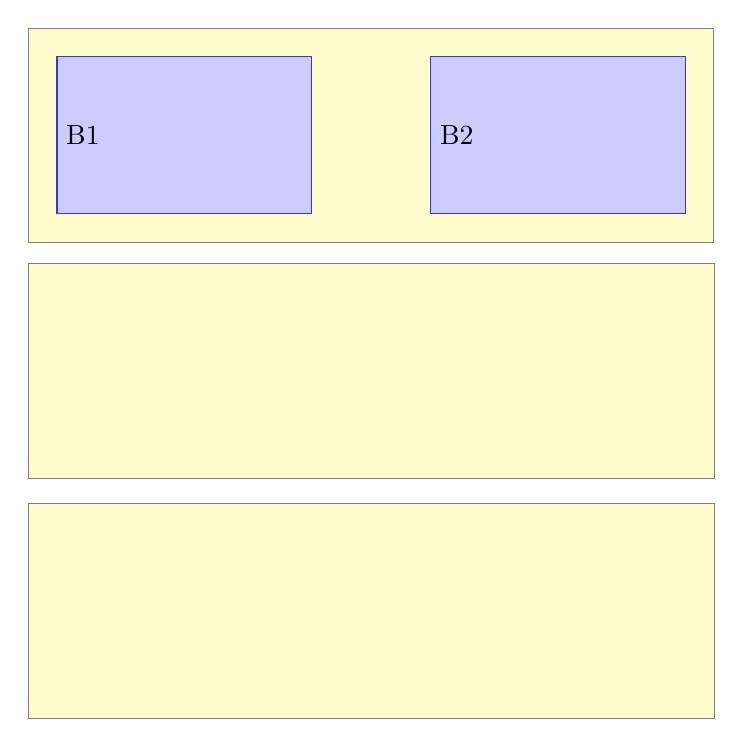
\begin{tikzpicture}
		\node[block]                (B1) {B1};
		\node[block, right = of B1] (B2) {B2};

		\begin{pgfonlayer}{background}
			\node[module, fit = (B1) (B2)] (F) { };
		\end{pgfonlayer}

		\filldraw [draw=black!50,fill=yellow!20] ([yshift=-3cm]F.south west) rectangle ([yshift=-3cm]F.north east);

		\draw let
		\p1=(F.south west),\p2=(F.north east),\n1={(\x2-\x1)},\n2={(\y2-\y1)} in
		node[module,minimum width=\n1,minimum height=\n2,below=3.3cm of F.south] (F2) {};

	\end{tikzpicture}

\end{document}º